\documentclass[11pt, a4paper]{article}

\usepackage[margin=1in]{geometry}
\usepackage{hyperref}
\usepackage{graphicx}
\usepackage{titlesec}
\usepackage{booktabs}
\usepackage{amsmath}

\titleformat{\section}{\large\bfseries}{\thesection}{1em}{}
\titleformat{\subsection}{\normalsize\bfseries}{\thesubsection}{1em}{}

\title{\textbf{Analysis of Performance Drop After Copy-Paste Augmentation}}
\author{Huy Khanh Tran}

\begin{document}
\maketitle

\section{Brief Summary}
This report explains why the copy-paste augmented datasets reduce performance. The short answer is simple: the new samples do not clearly align with the test distribution, and in Global Wheat Head the score-guided version is even farther from test than random copy-paste.

\section{Research Problem}
The main question is whether the augmented images remain valid training samples or become distribution-shifted samples that hurt generalization. This is the problem I am investigating now because performance drops after adding copy-paste augmentation.

To study that, I used a frozen YOLOv8s backbone, extracted image-level embeddings from the P5 feature map with global average pooling, and compared original training images, random augmented images, score-guided augmented images, and test images.

\section{Scoring}
The scoring system is the bridge between the baseline model and augmentation. It uses the model's own failure behavior to rank difficult objects and images. Low-confidence predictions measure object difficulty, and optimal-threshold predictions measure false positives. The idea is to select hard samples more often. The problem is that harder samples are not automatically closer to the test distribution.

\section{Visual Comparison}
Figure~\ref{fig:aug_compare} shows the same style of augmented-vs-base comparison used in the notebook viewer. It is the clearest visual check for whether the new image still looks like a plausible sample from the original dataset.

\begin{figure}[htbp]
    \centering
    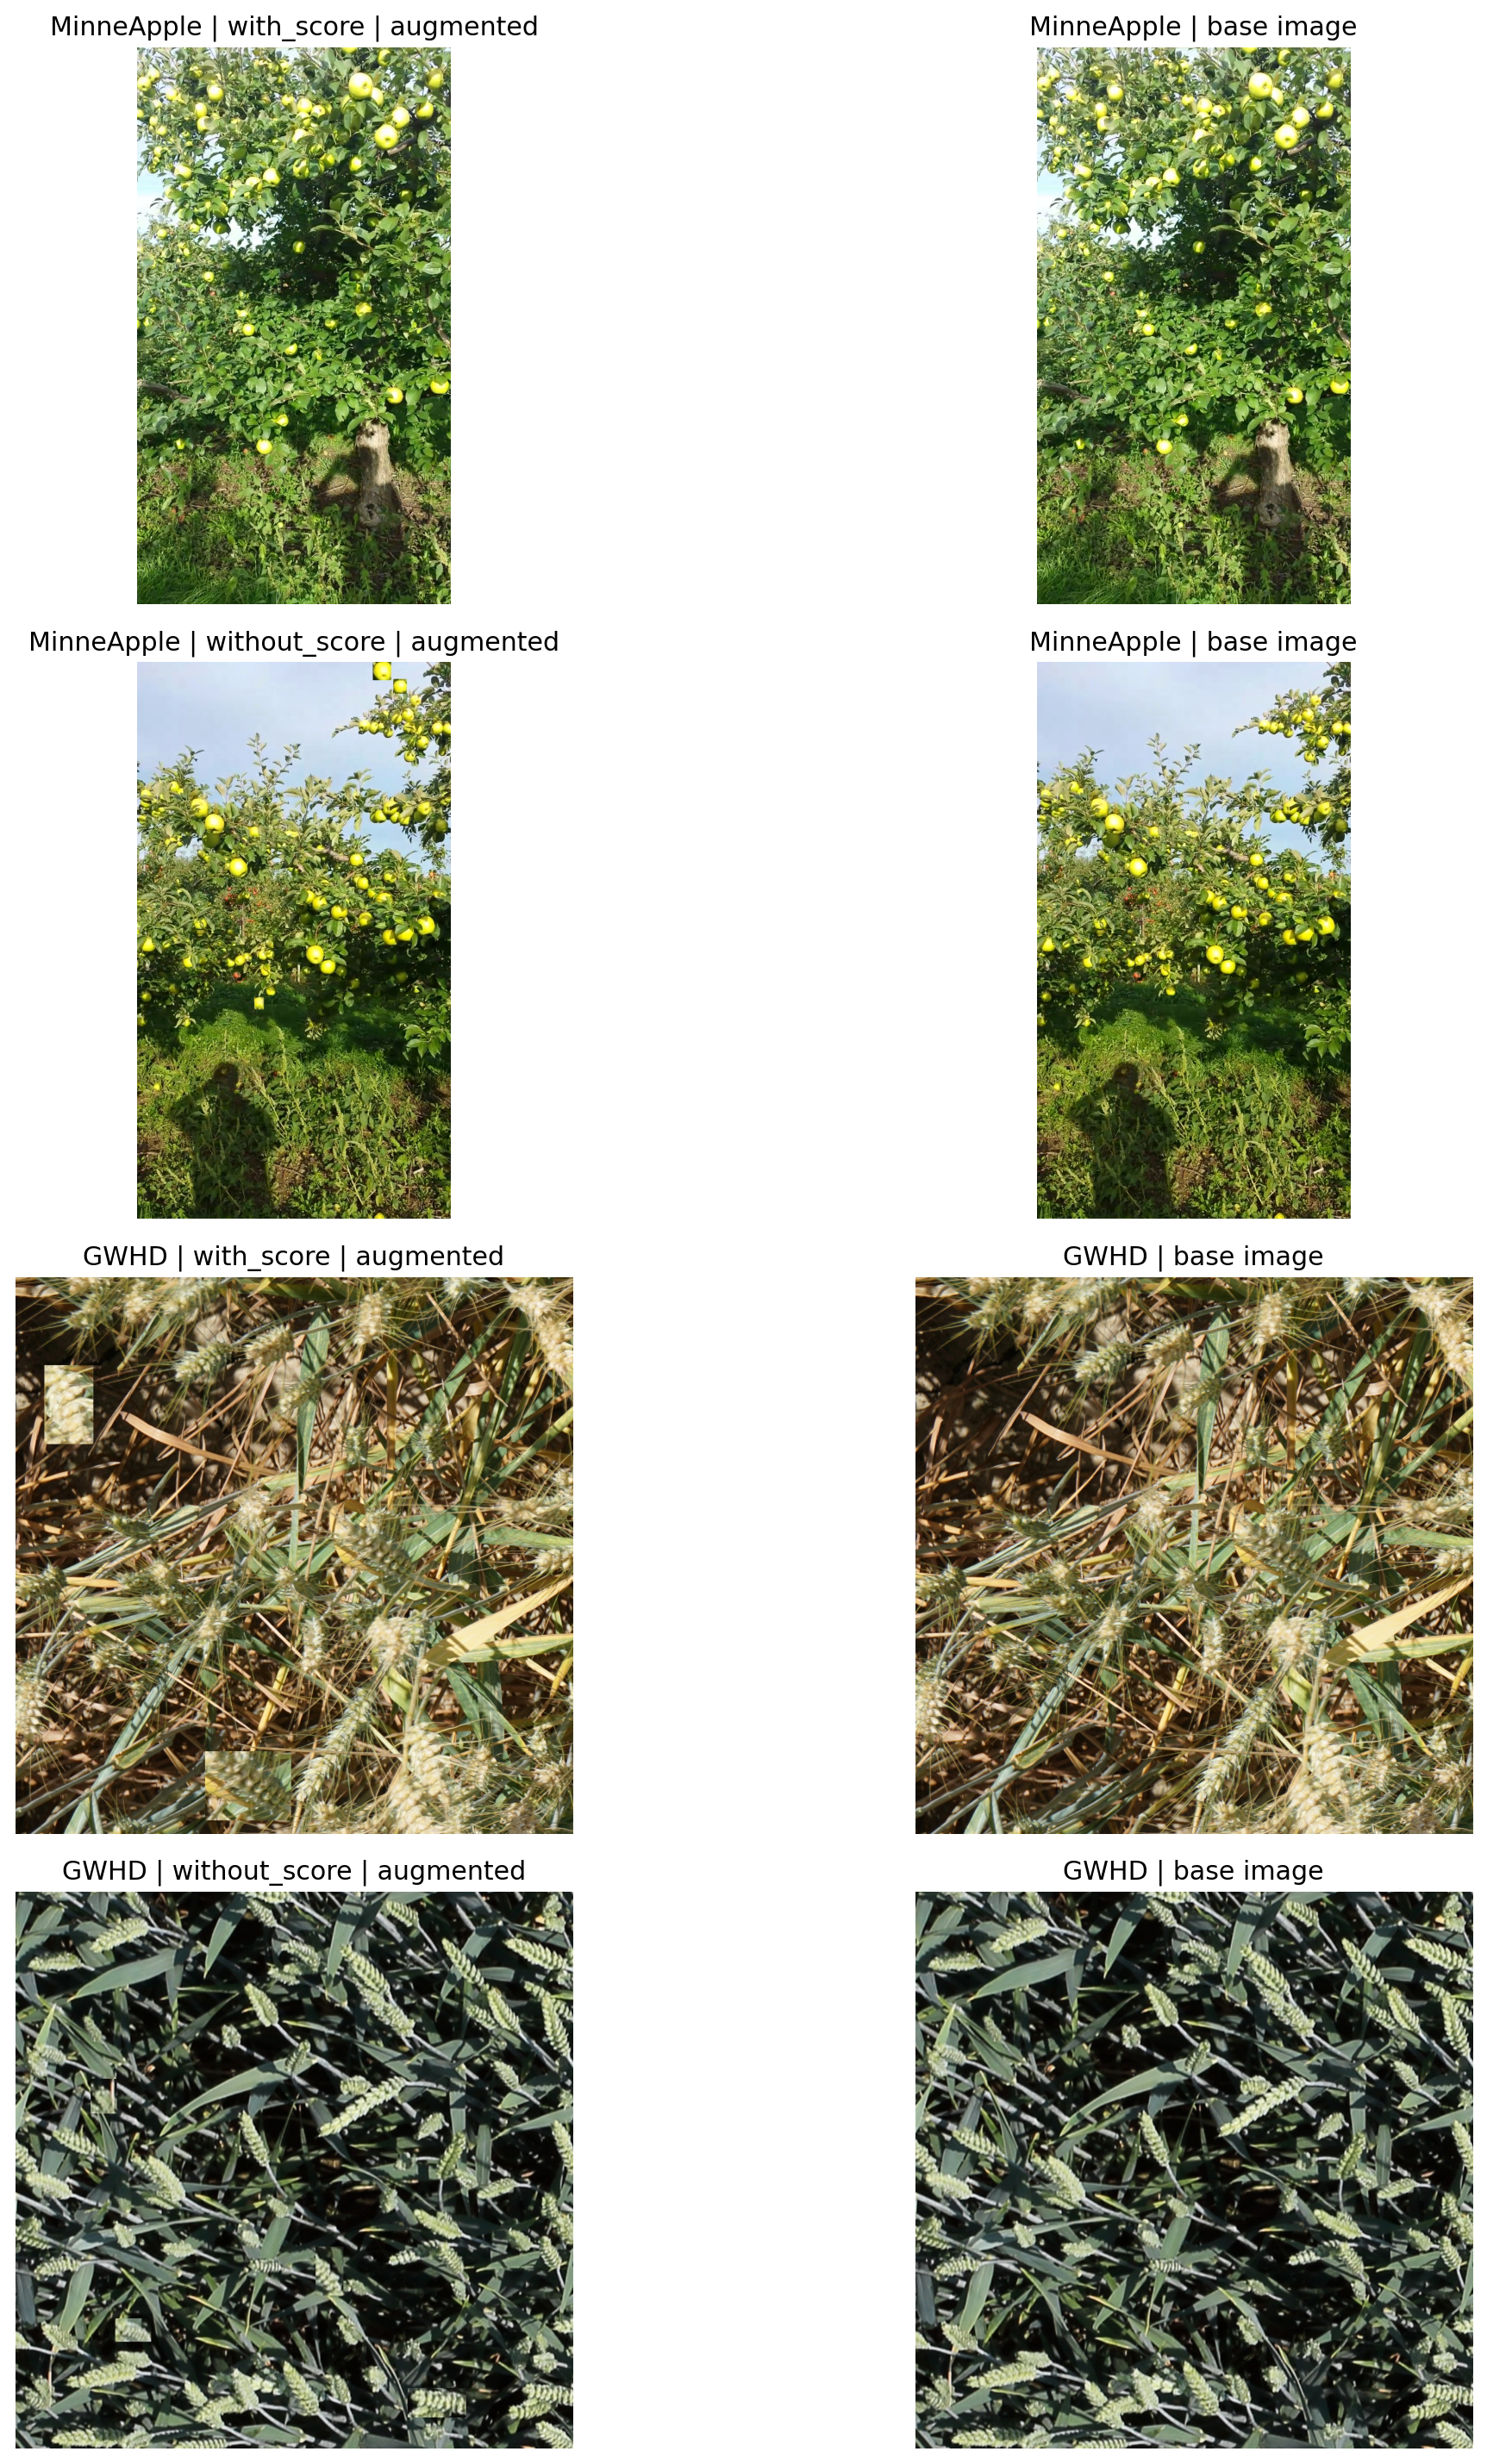
\includegraphics[width=0.95\textwidth,height=0.55\textheight,keepaspectratio]{figures/augmentation_comparison_minneapple_gwhd.png}
    \caption{Representative augmented-vs-base comparison for MinneApple and Global Wheat Head.}
    \label{fig:aug_compare}
\end{figure}

\section{Feature-Space Analysis}
This is the key result.

\subsection{MinneApple}
MinneApple uses same-image copy-paste. The feature-space plot shows that original train, random augmentation, and score-guided augmentation stay close to each other, while test is separated. So the augmented images are not obvious outliers, but they also do not move toward the test distribution. The mechanism is still not fully clear.

\subsection{Global Wheat Head}
Global Wheat Head is more problematic because cross-image copy-paste mixes domains. The centroid distances are:
\begin{itemize}
    \item original train $\rightarrow$ test: 16.8058
    \item augmented random $\rightarrow$ test: 16.2602
    \item augmented score $\rightarrow$ test: 17.3665
\end{itemize}

The sharp observation is that score-guided augmentation is the farthest from test. That matches the performance drop. What is still not clear is the exact causal mechanism: whether the drop is caused by density, domain mixing, poor placement, or the scoring rule itself.

\section{Conclusion}
The conclusion is direct: the current copy-paste augmentation does not reliably improve the training distribution, and score-guided selection is not the fix. For MinneApple, the samples stay close to the training manifold but still do not improve test alignment. For Global Wheat Head, score-guided augmentation is clearly the most misaligned with test. So the performance drop is consistent with distribution mismatch, but the exact reason is still not fully resolved.

\section{Detailed Experimental Setup}
This final part records how the experiments were made and what they produced.

\subsection{Experiment sources}
\begin{itemize}
    \item MinneApple result root: \texttt{results/12\_multiseed\_score\_vs\_noscore\_copy\_paste\_exp\_apple\_withaug}
    \item Global Wheat Head result root: \texttt{results/13\_multiseed\_score\_vs\_noscore\_copy\_paste\_exp\_global\_wheat\_head}
    \item Feature analysis notebooks: \texttt{notebooks/augmentation\_feature\_space\_outlier\_analysis.ipynb} and \texttt{notebooks/augmentation\_feature\_space\_outlier\_analysis\_gwhd.ipynb}
\end{itemize}

\subsection{Configuration table}
\begin{center}
\small
\begin{tabular}{@{}lll@{}}
\toprule
\textbf{Setting} & \textbf{MinneApple} & \textbf{Global Wheat Head} \\
\midrule
Backbone & YOLOv8s & YOLOv8s \\
Feature level & P5 & P5 \\
Embedding method & GAP over feature map & GAP over feature map \\
Seed count & 1 for feature analysis, 3 for comparison & 3 \\
Copy-paste mode & same-image-only for MinneApple & cross-image for GWHD \\
Augmentation variants & random vs score-guided & random vs score-guided \\
Comparison target & test distribution distance & test distribution distance \\
\bottomrule
\end{tabular}
\end{center}

\subsection{Result table: Global Wheat Head}
\begin{center}
\small
\begin{tabular}{@{}lrrr@{}}
\toprule
\textbf{Condition} & \textbf{COCO\_AP} & \textbf{AP50} & \textbf{AP75} \\
\midrule
Baseline mean & 0.50699 & 0.92226 & 0.49071 \\
With-score mean & 0.48367 & 0.90454 & 0.45494 \\
Without-score mean & 0.48570 & 0.90476 & 0.45556 \\
\midrule
With-score $\Delta$ vs baseline & -0.02332 & -0.01773 & -0.03578 \\
Without-score $\Delta$ vs baseline & -0.02129 & -0.01750 & -0.03515 \\
\bottomrule
\end{tabular}
\end{center}

\subsection{Result table: MinneApple}
\begin{center}
\small
\begin{tabular}{@{}lrrrrrr@{}}
\toprule
\textbf{Condition} & \textbf{COCO\_AP} & \textbf{COCO\_AP50} & \textbf{COCO\_AP75} & \textbf{AP\_small} & \textbf{AP\_medium} & \textbf{AP\_large} \\
\midrule
Baseline & 0.4472 & 0.7743 & 0.4637 & 0.3075 & 0.5996 & 0.7191 \\
Random copy-paste & 0.4362 & 0.7695 & 0.4532 & 0.2903 & 0.5933 & 0.7158 \\
Score-guided copy-paste & 0.4280 & 0.7882 & 0.4288 & 0.2979 & 0.5748 & 0.6271 \\
\bottomrule
\end{tabular}
\end{center}

\subsection{Observation from the tables}
On both datasets, the augmented results are below the baseline on COCO\_AP. On Global Wheat Head, the score-guided variant is consistently worse than random. On MinneApple, score-guided copy-paste gives the weakest AP75. That is enough to support the main claim, but not enough to explain every detail of the failure.

\section{Appendix}
The notebook outputs and the raw experiment summaries used for this report are stored under the corresponding \texttt{results/} directories.

\end{document}
